\id{ҒТАМР 06.52.13}{https://doi.org/10.58805/kazutb.v.4.25-547}

\begin{articleheader}
\sectionwithauthors{А.К.Ибраева, Д.М. Акишева, М.С. Искакова}{ӨНЕРКӘСІПТІК КЕШЕНДІ БАСҚАРУДА ЖОСПАРЛАУ МЕН БОЛЖАУДЫ
ҰЙЫМДАСТЫРУДЫ ЖЕТІЛДІРУ}

{\bfseries А.К.Ибраева\textsuperscript{\envelope }, Д.М. Акишева, М.С. Искакова}
\end{articleheader}
\begin{affiliation}

«Семей қаласының Шәкәрім атындағы Университеті» КеАҚ,Семей, Казақстан

\raggedright {\bfseries \textsuperscript{\envelope }}Корреспондент-автор:\href{mailto:zeretai@mail.ru}{\nolinkurl{zeretai@mail.ru}}
\end{affiliation}

Қазақстанның өнеркәсіптік кешенін басқаруды жоспарлау мен болжауды
ұйымдастыруды жетілдіру мәселелері қарастырылған.Ұзақ мерзімді жоспарлау
және болжамдау процестерінің сақталуы, өнеркәсіптік кешенді басқарудағы
жоспарлы - болжамдық қызметті жетілдіру бойынша мемлекеттік органдардың
функциялары ашылды.Зерттеу нәтижелері бойынша қорытындылар жасалды және
өнеркәсіптік кешенді басқаруда жоспарлауды ұйымдастыруды жетілдіру
бойынша шаралар ұсынылады.Жүргізілген зерттеу негізінде келесідей
қорытынды жасауға болады: өнеркәсіптік кешендегі жоспарлы-болжамдық
қызмет елдің индустриялық-инновациялық дамуының ұзақ мерзімді
стратегиялық бағдарламаларын орындаудың кілті болып табылады;
жоспарлы-болжамдық қызмет күрделі процесс болып табылады, оның сапасына
өнеркәсіпті және тұтастай алғанда экономиканың мемлекеттік секторын
дамытудың тиімділігі тәуелді болады; өнеркәсіп кешенінде
жоспарлы-болжамды қызметті реттеуді Қазақстан Республикасы Индустрия
және жаңа технологиялар министрлігіжүзеге асырады.Бұл органға
жоспарлы-болжамдық органдар жүйесін жетілдіру жөніндегі функциялар
кіреді.Институттың функцияларына өнеркәсіпті дамытуды үйлестіру және
өнеркәсіп салаларын дамытудың негізгі үрдістерін болжау да
жатады.Алайда, өнеркәсіптік кешенді басқаруда жоспарлау мен болжауды
ұйымдастыруды жетілдіру мақсатында мынадай іс-шаралар жүргізу
қажет:елдің әрбір аймағында өңірдің өнеркәсіптік кешенін басқаруды
жоспарлау және болжау қызметтерін ұсыну жөнінде тәуелсіз кеңестік
орталықтар құру,тәуелсіз кеңестік орталықтардың негізінде тәуелсіз
сараптамалар жүргізу жөніндегі сараптамалық мекемелер құру,өңірлік
өнеркәсіпті дамытудың стратегиялық бағдарламаларын іске асыру жөніндегі
жоспарларды, өңірлік болжамдарды, жоспарларды, бағдарламаларды әзірлеуге
кәсіпорындардың мамандарын тарту.

{\bfseries Түйін сөздер:} жоспарлау, болжамдау, индустриялық даму,
өнеркәсіптік кешен.
\begin{articleheader}

{\bfseries СОВЕРШЕНСТВОВАНИЕ ОРГАНИЗАЦИИ ПЛАНИРОВАНИЯ И ПРОГНОЗИРОВАНИЯ В
УПРАВЛЕНИИ ПРОМЫШЛЕННЫМ КОМПЛЕКСОМ}

{\bfseries А.К.Ибраева\textsuperscript{\envelope }, Д.М. Акишева, М.С. Искакова}
\end{articleheader}
\begin{affiliation}

НАО университет имени Шакарима города Семей, Семей, Казақстан,

е-mail: zeretai@mail.ru
\end{affiliation}

Рассмотрены вопросы совершенствования организации планирования и
прогнозирования управления промышленным комплексом Казахстана. По
результатам исследования предложены меры по совершенствованию
организации планирования в управлении промышленным комплексом. На
основании проведенного исследования можно сделать следующие выводы:
планирование и прогнозирование деятельности в промышленном комплексе
являются залогом долгосрочного краткосрочные стратегические программы
Планирование и прогнозирование деятельности - это сложный процесс, от
качества которого зависит эффективность развития отрасли и
государственного сектора экономики в целом; Плановую и прогнозируемую
деятельность в промышленном комплексе регулирует Министерство индустрии
и новых технологий Республики Казахстан. Этот орган включает в себя
функции по совершенствованию системы органов планирования и
прогнозирования. Для совершенствования организации прогнозирования
необходимо принять следующие меры: создание независимых консультационных
центров по планированию и предоставлению прогнозных услуг в каждом
регионе страны; привлечение специалистов предприятий к разработке
региональных прогнозов, планов, программ.

{\bfseries Ключевые слова:} планирование, прогнозирование, промышленное
развитие, промышленный комплекс.
\begin{articleheader}

{\bfseries IMPROVING THE ORGANIZATION OF PLANNING AND FORECASTING IN THE
MANAGEMENT OF THE INDUSTRIAL COMPLEX}

{\bfseries A.K. Ibraeva\textsuperscript{\envelope }, D.M. Akisheva, M.S. Iskakova}
\end{articleheader}
\begin{affiliation}

Shakarim University of Semey, Semey, Kazakhstan,

е-mail: \href{mailto:zeretai@mail.ru}{\nolinkurl{zeretai@mail.ru}}
\end{affiliation}

The issues of improving the organization of planning and forecasting of
the management of the industrial complex of Kazakhstan are considered.
Based on the results of the study, measures are proposed to improve the
organization of planning in the management of the industrial complex.
Based on the study, the following conclusions can be made: planning and
forecasting activities in the industrial complex are the key to
long-term strategic programs Planning and forecasting activities are a
complex process, the quality of which depends on the effectiveness of
the development of industry and the public sector of the economy as a
whole; The Ministry of Industry and New Technologies of the Republic of
Kazakhstan regulates the planned and forecasted activities in the
industrial complex. This body includes the functions of improving the
system of planning and forecasting bodies. In order to improve the
organization of forecasting, it is necessary to take the following
measures: establishment of independent consulting centers for planning
and providing forecasting services in each region of the country,
establishment of expert institutions for independent expertise on the
basis of independent consulting centers; , involvement of specialists of
enterprises in the development of regional forecasts, plans, programs.

{\bfseries Keywords:} planning, forecasting, industrial development,
industrial complex.
\begin{multicols}{2}

{\bfseries Кіріспе} Өнеркәсіптік кешенді басқаруда жоспарлауды
ұйымдастыруды жетілдіру аймақтар үшін де, жалпы мемлекет үшін де
проблемалық міндет болып табылады. Көрсетілген проблема өнеркәсіптік
кешенді басқару жөніндегі уәкілетті мемлекеттік органдардың жоспарлы -
болжамдық қызметі жүйелерінің тиімділігін арттыру жолымен шешіледі.

Зерттеудің мақсаты инновациялық технологиялар негізінде өнеркәсіптік
кешенді басқаруда жоспарлау мен болжауды ұйымдастырудың әдістемелік
негіздерін әзірлеу және тиісті ұсыныстар әзірлеу болып табылады.

Қазақстанның өнеркәсіптік кешені үшін қазіргі кезеңде ұзақ мерзімді
жоспарлауды дамыту неғұрлым тиімді болып табылады.Мұның себептері болып
өнеркәсіптік кешенде жоспарлау мақсаттарына қол жеткізу үшін
индикаторлар жүйесін әзірлеу және бекіту табылады.Сонымен қатар,
өнеркәсіптік кешенді ұзақ мерзімді жоспарлау аймақтық деңгейде де,
республикалық деңгейде де болуы мүмкін.

Бүгінгі таңда нарықтық экономика және экономиканың қаржы секторының
тұрақсыздығы жағдайында өнеркәсіптік өндірісті басқаруды жоспарлау
күрделі және тәуекелді процесс болып табылады.Перспективалық жоспарды
сапалы әзірлеу келесілермен байланысты өнеркәсіптік кешеннің
стратегиялық мәселелерін іске асырады:

- өндіріс құрылымының сапа менеджментін арттыру;

- өнеркәсіпке инновацияларды уақтылы енгізумен;

- тиімді интеграцияланған құрылымдарды құру;- өзге де стратегиялық
мәселелермен айналысуға тиіс.

Алайда, сапалы жоспарды әзірлеу өнеркәсіптік кешенді болжау жүйесінсіз
мүмкін емес.Бұл жағдайда болжау жүйесінде нақты және бағытталған болжау
процестері болады.Болжамның өзі екі кезеңнен тұрады.Бірінші кезең
мемлекеттің немесе аймақтың ғылыми -- техникалық прогресі өнеркәсіптің
болжамын әзірлеуді қамтиды. Екінші кезеңде техника мен технология
динамикасының неғұрлым перспективалы бағыттарының болжамы жасалады,
сондай-ақ басым өндірістер айқындалады.

{\bfseries Материалдар мен әдістер.} Бұдан әрі технологияларды, техниканы
зерттеу және басым өндірістерді таңдау негізінде өндірістік кешенді
дамытудың ұзақ мерзімді жоспары жасалады.

Ұзақ мерзімді жоспарды іске асыру оны іске асыру әдістерін таңдауға
байланысты. Практикада ұзақ мерзімді жоспардың тапсырмаларын бірнеше
кезеңге саралау әдісі бар (негізінен кезең жылдарға бөлінеді).Осылайша,
жоспарлау процесінің үздіксіздігі, нарықтық жағдайда өзгерістер болса,
жоспарларды уақтылы түзету қамтамасыз етіледі.

Кәсіпорында жоспарлау және болжау мәселелерінің теориялық және
әдістемелік аспектілері келесідей авторлардың жұмыстарында
қарастырылған: Л.Е. Басовский, Ф. Л. Шаров, Т. Г. Морозова, А. В.
Пикулькин, В. И. Кушлин, Н. А. Волгин, Р. Гусейнов {[}1-5{]} және
басқалар. Сонымен бірге нарықтық экономика жағдайында әдебиеттерде,
өнеркәсіптік кешенді басқаруды дамытуды стратегиялық болжау мен
жоспарлаудың теориялық, әдіснамалық сипатының бірқатар
аспектілеріжеткіліксіз қарастырылған.

Жоғарыда көрсетілген әдістемені қолдану процесінде уәкілетті мемлекеттік
органдар тапсырмаларды кезеңдерге бөле отырып, ұзақ мерзімді жоспар
жасайды.Бұл ретте жоспарды іске асырудың әрбір кезеңі үшін орындалатын
жұмыстардың көлемін айқындау маңызды болып табылады. Сондай - ақ,
берілген жұмыстарды орындауға тағайындалған адам үшін қажетті
мерзімдерді анықтау қажет {[}6{]}.

Нарықтың қатал шарты отандық өнім өндірушілердің бәсекелік қауқарын
нығайтуды, өнімдерінің бәсекелік қыспақтарға төтеп берерлік қабілетін
арттыруды, ішкі және сыртқы нарықтарда сұранысы жоғары өнім өндіруге
тиімді әсері бар тетіктерді айқындауды және сол арқылы мемлекеттің
қауіпсіздігін қамтамасыз ету мәселесін шешуді қажет етеді. Ұлттық
экономикадағы нақты саланың дамуын қамтамасыз етуде, отандық
өндірушілердің өнімдерін әлемдік нарықтың сұранысына сәйкестендіру
бағытында атқарылатын іс-шаралардың тобына шығарылатын өнімдердің
бәсекелік қабілетін қамтамасыз ету мәселесін жатқызуға болады.

Алайда, мұндай жоспарды құру өнеркәсіптік кешенді басқарудағы тиімді
жоспарлау және жоспарлау іс - шараларынсыз мүмкін емес.
Жоспарлы-болжамдық қызметті жетілдіру мақсатында екі бағытта өзгерістер
жүргізу қажет:

- жоспарлы-болжамдық органдар жүйесін жетілдіру;

- жоспарлы-болжамдық құжаттардың құрылымын оңтайландыру.

Бірінші бағытта барлық деңгейдегі жоспарлы - болжамдық органдар
құрылымында кеңестік аппараттың рөлін күшейту басым міндет болып
табылады.Мемлекеттік деңгейде жоспарлы-болжамдық үдерісті іске асыруда
негізгі рөлді Қазақстан Республикасы өнеркәсіп және құрылыс
министрлігінің, ал аймақтық деңгейде - облыстық және аудандық әкімдіктер
жанындағы құрылымдық басқармалар мен бөлімдер жүзеге асырады.

Қазақстанда индустриялық-инновациялық даму процестерін жоспарлаумен және
болжаумен, сондай - ақ өнеркәсіптік кешенді дамытудың стратегиялық
бағдарламаларының қазіргі жай - күйін талдаумен "Қазақстандық
индустрияны дамыту институты" АҚ ("ҚИДИ" АҚ), бұдан әрі - институт
айналысады. {[}7{]}.

Өнеркәсіпті басқаруда кәсіпорынның бәсекеге қабілеттілігі
детерминанттардың екі негізгі тобы ретінде көрінетінін айқындап алған
жөн.(сурет. 1).
\end{multicols}


\begin{figure}[H]
	\centering
	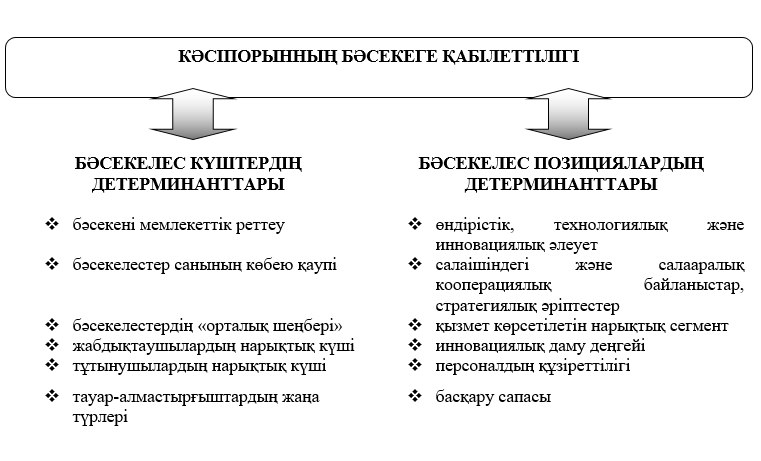
\includegraphics[width=0.8\textwidth]{media/ekon/image1.1}
	\caption*{1-сурет -- Өнеркәсіптік кәсіпорынның бәсекеге қабілеттілік
	детерминанттары}
\end{figure}

\begin{multicols}{2}

Ұйымның бәсекеге қабілеттілігін зерттеген кезде, осы екі факторлар
тобына баса назар аудару керек.

{\bfseries Нәтижелермен талқылау.} ҚИДИ" АҚ Жарғысына сәйкес институт келесі
қызмет түрлерін жүзеге асырады:

1)қазақстандық өндірістерді жаңғырту және әртараптандыру,инновациялық
саясат саласында зерттеулер жүргізу,өнеркәсіптің өңдеушісекторларының
және туризм индустриясының бәсекеге қабілеттілігін арттыру;

2) өнеркәсіп пен туризм индустриясын дамытудың теориялық, әдіснамалық
және практикалық мәселелеріне зерттеулер жүргізу;

3) өнеркәсіп салаларын, туризм индустриясын қайта құрылымдаудың және
салааралық кооперацияны дамытудың экономикалық факторларына зерттеулер
жүргізу, өнеркәсіптегі, туризм индустриясындағы қайта құрылымдау мен
салааралық кооперацияны ынталандыру және қолдау жөніндегі шаралар
әзірлеу;

4) өндірістерді, туризм объектілерін әртараптандырудың және кластерлерді
дамытудың экономикалық факторларына зерттеулер жүргізу, өндірістерді,
туризм объектілерін әртараптандыруды ынталандыру және қолдау,
кластерлерді дамыту жөнінде шаралар әзірлеу;

5) туризмнің жаңа өндірістері мен объектілерін құрудың
техникалық-экономикалық негіздемелерін және аумақтық орналастыру
схемаларын, инвестициялық жобалар бойынша сараптамалық қорытындыларды,
өңірлік өндірістік жүйелерді, туристік және өнеркәсіптік инфрақұрылымды
қалыптастыру және дамыту тұжырымдамаларын әзірлеу;

6) Қазақстанның өнеркәсіп салалары мен туризм индустриясы сегменттерінің
әлемдік өндірістік - шаруашылық жүйелерге интеграциялануын қамтамасыз
ету және халықаралық туризмді дамыту жөнінде ұсыныстар дайындау;

7) өнеркәсіп пен туризм индустриясын дамыту мәселелері бойынша заң
жобаларын, салалық бағдарламаларды, мемлекеттік органдардың
мастер-жоспарлары мен іс - шаралар жоспарларын әзірлеуге қатысу;

8)туризм өнеркәсібі мен индустриясын дамытудың экономикалық
көрсеткіштерін бағалау және бақылау үшін әдістемелер мен практикалық
нұсқаулықтар әзірлеу;

9) өндірістерді оңтайлы орналастыру, кластерлерді дамыту, арнайы
экономикалық және индустриялық аймақтар құру жөнінде ұсыныстар дайындау;

10) өнеркәсіп салалары мен туризм индустриясы дамуының негізгі
үрдістерін болжау;

11) экономиканың басым секторларын дамыту саласында
ақпараттық-талдамалық және кеңестік қызметтер көрсету;

12) индустриялық-инновациялық қызмет саласындағы салалық
бағдарламалардың орындалу мониторингіне қатысу;

13) индустриялық - инновациялық қызметті мемлекеттік қолдау саласындағы
уәкілетті органға басым тауарлар мен көрсетілетін қызметтердің бірыңғай
картасын әзірлеу және өзектілендіру бойынша қызметтер көрсету;

14) индустриялық - инновациялық қызметті мемлекеттік қолдау саласындағы
уәкілетті органға Индустрияландыру картасының экономикалық тиімділігін
талдау бойынша қызметтер көрсету;

15) озық технологияларды тарта отырып, қазақстандық кәсіпорындар мен
ұйымдарға жаңа өндірістер құруға жәрдемдесу {[}8{]}.

Институт функцияларын талдау, «ҚИДИ» АҚ экономиканың басым секторларын
дамыту және өнеркәсіп салаларын дамытудың негізгі басымдықтарын болжау
саласында консультация беруді жүзеге асыратынын көрсетеді.

Бұл функциялар өңірлер бойынша жоспарлы - болжамдық құжаттарды әзірлеу
кезінде, қызмет көрсету жөніндегі институт мамандарының жеке қатысуының,
сондай - ақ Қазақстанның электрондық үкіметінің порталындағы "Интернет"
жүйесі арқылы қашықтықтан байланыстың қажеттілігін көздейді.

Жоспарлы-болжамды қызметті жетілдірудің екінші бағытын іске асыру
мақсатында институт мынадай қызметтерді іске асырады:

болжау және жоспарлау бағдарламаларын және ілеспе құжаттаманы жасау;

- мемлекеттік органдардың жергілікті жерде жоспарлы-болжамды құжаттарын
жасауды үйлестіру;

осы әзірлемелердің теңдігін қамтамасыз ету және оларды бірыңғай
болжамда, өңірдің әлеуметтік-экономикалық даму жоспарында жинақтау
{[}9{]}.

Алайда, іс жүзінде институт мамандарының және жергілікті жерлердегі
мемлекеттік органдардың жоспарлы-болжамды қызметін тәуелсіз бақылау
немесе кеңес беру бойынша проблемалар айқын болып отыр.

{\bfseries Қорытынды.} Жүргізілген зерттеулер нәтижесінде келесідей
қорытынды жасауға болады:

1) өнеркәсіптік кешендегі жоспарлы-болжамды қызмет елді
индустриялық-инновациялық дамытудың ұзақ мерзімді стратегиялық
бағдарламаларын орындаудың кілті болып табылады;

2)жоспарлы-болжамды қызмет күрделі процесс болып табылады, оның
сапасынан жалпы экономиканың өнеркәсіптік және мемлекеттік секторын
дамытудың тиімділігі тәуелді болады;

3) Қазақстанның өнеркәсіптік кешеніндегі жоспарлы-болжамды қызметті
реттеуді Қазақстан Республикасы Индустрия және жаңа технологиялар
министрлігінің Өнеркәсіп комитеті жүзеге асырады. Бұл органға жоспарлау
және болжау органдарының жүйесін жетілдіру функциялары кіреді;

4)Қазақстанда жоспарлы - болжамды құжаттаманы оңтайландыру бойынша
кеңестңк қызметтерді жүзеге асыратын орган «Қазақстандық индустрияны
дамыту институты» АҚ болып табылады. Институт функцияларына өнеркәсіптің
дамуын үйлестіру және өнеркәсіп салалары дамуының негізгі үрдістерін
болжау кіреді.

Алайда, өнеркәсіптік кешенді басқаруда жоспарлау мен болжауды
ұйымдастыруды жетілдіру мақсатында келесідей іс-шараларды жүргізу қажет:

1) елдің әрбір өңірінде аймақтың өнеркәсіптік кешенін басқаруды
жоспарлау және болжау қызметтерін ұсыну жөнінде тәуелсіз кеңестік
орталықтар құру;

2) тәуелсіз кеңестік орталықтардың негізінде аймақтық өнеркәсіпті
дамытудың стратегиялық бағдарламаларын іске асыру, тәуелсіз сараптамалық
жоспарларды өткізу жөніндегі тәуелсіз сараптамалар жүргізетін мекемелер
құру;

3) өңірлік болжамдарды, жоспарларды, бағдарламаларды әзірлеуге
кәсіпорындардың мамандарын тарту;

4) өңірлерді ақпаратпен қамтамасыз ету мақсатында, негізгі құрал ретінде
өнеркәсіп комитетінің жеке электрондық сайтын енгізу қажет.

Сайттың функциясына кең ауқымды талдамалық, болжамдық, нормативтік -
құқықтық ақпарат, сондай-ақ мемлекеттік сатып алу туралы ақпарат кіреді.

Жалпы алғанда, өнеркәсіптік кешенді басқарудағы жоспарлау мен болжауды
мемлекеттік реттеу тек аналитикалық ғана емес, сонымен бірге
оңтайландыруды да болжау мен жоспарлаудың жаңа озық жүйелерін уақтылы
енгізуді қамтамасыз етеді.
\end{multicols}

\begin{center}
{\bfseries Әдебиеттер}
\end{center}

\begin{references}

1. Бригхем Ю., Гапенски Л. Финансовый менеджмент, 1997,-497 с.ISBN 0 03
075482-8

2.АнсоффИ. Стратегическоеуправление.-М.Экономика.-1989.- 520 с. ISBN
5-282-00652-9.

3.Томпсон А.А., СтриклендА.Дж. Стратегический менеджмент. Искусство
разработки стратегии/ Перевод с английского под редакцией Л. Г. Зайцева,
М.И. Соколовой.-

М: Банки и биржи, ЮНИТИ, 1998. - 576 с. ISBN 0-256-15027-3.ISBN
5-85173-059-5

4.Алимбаев, К.С. Айнабек, С.Н. Ахметов и др.Основы управления
рыночной~экономики - Караганда: Болашак-Баспа, 2002. - 340 с.
-~ISBN~9965-528-39-X

5.Зиядин С.Т. Некоторые проблемы развития малого предпринимательства
Казахстана// Деньги и кредит.-2014.-№ 6. - С.72-74

6.Фелештин В.И. Современные подходы к определению понятия
«конкурентоспособность предприятия» // Вестник Белгородского
университета кооперации, экономики и права.- 2015.- № 3.- С.401-409

7. Хаустов А.А. Отраслевые кластеры как формат интеграции регионов СКФО
в мирохозяйственные связи.// Экономика и предпринимательство.-2016.- №
9.- С.198-201

8.Тарасенко В. В. Территориальные кластеры: семь инструментов
управления.М., 2015.- 201 с. ISBN978-5-9614-4705-7

9.Матковская Я.С. Кластеры: анализ происхождения, современные формы
институсионализасии и математические модели // Финансовая аналитика:
проблемы и решения//
~\href{https://www.fin-izdat.ru/journal/fa/}{Финансовая аналитика:
проблемы и решения}.-2014.-№ 17..- S.2-12. [in Russ.]
10. Колесов Э.В. Методы управления промышленным комплексом региона//
Вестник СГАУ имени М.Решетнева -2018.- № 1.- С.171-181

\url{https://cyberleninka.ru/article/n/metody-upravleniya-promyshlennym-kompleksom-regiona}
\end{references}

\begin{center}
{\bfseries References}
\end{center}

\begin{references}

1.Brighem Ju., Gapenski L. Finansovyj menedzhment, 1997,-497 s. ISBN 0
03 075482-8.{[}in Russ.{]}

2.Ansoff I. Strategicheskoe upravlenie.-M.Jekonomika.-1989.- 520 s. ISBN
5-282-00652-9.{[}in Russ.{]}

3.Tompson A.A., Striklend A.Dzh. Strategicheskij menedzhment. Iskusstvo
razrabotki strategii/ Perevod s anglijskogo pod redakciej L. G. Zajceva,
M.I. Sokolovoj.- M: Banki i birzhi, JuNITI, 1998. - 576 s. ISBN
0-256-15027-3 (angl.) ?ISBN 5-85173-059-5 (russk.) {[}in Russ.{]}

4.Alimbaev, K.S. Ajnabek, S.N. Ahmetov i dr. Osnovy upravlenija
rynochnoj jekonomiki - Karaganda: Bolashak-Baspa, 2002. - 340 s. - ISBN
9965-528-39-X. {[}in Russ.{]}

5.Zijadin S.T. Nekotorye problemy razvitija malogo
predprinimatel' stva Kazahstana// Den' gi
i kredit.-2014.-№ 6. - S.72-74. {[}in Russ.{]}

6.Feleshtin V.I. Sovremennye podhody k opredeleniju ponjatija
«konkurentosposobnost'{} predprijatija» // Vestnik
Belgorodskogo universiteta kooperacii, jekonomiki i prava.- 2015.- № 3.-
S.401-409. {[}in Russ.{]}

7. Haustov A.A. Otraslevye klastery kak format integracii regionov SKFO
v mirohozjajstvennye svjazi.// Jekonomika i
predprinimatel' stvo.-2016.- № 9.- S.198-201. {[}in
Russ.{]}

8.Tarasenko V. V. Territorial' nye klastery:
sem'{} instrumentov upravlenija.M.,

2015.- 201 s. ISBN 978-5-9614-4705-7. {[}in Russ.{]}

9.Matkovskaja Ja.S. Klastery: analiz proishozhdenija, sovremennye formy

institusionalizasii i matematicheskie modeli // Finansovaja analitika:
problemy i reshenija// Finansovaja analitika: problemy i
reshenija.-2014.-№ 17.- S.2-12. {[}in Russ.{]}

10. Kolesov E.V. Metody upravleniya promyshlennym kompleksom regiona//
Vestnik SGAU imeni M.Reshetneva -2018.- № 1.- S.171-181 \url{https://cyberleninka.ru/article/n/metody-upravleniya-promyshlennym-kompleksom-regiona}
\end{references}
\begin{authorinfo}

\hspace{1em}\emph{{\bfseries Авторлар туралы мәліметтер}}

Ибраева А.К.- экономика ғылымдарының кандидаты,«Семей қаласының Шәкәрім
атындағы Университеті» КеАҚ, Семей, Казақстан, e-mail:
\href{mailto:ZEretai@mail.ru}{\nolinkurl{zeretai@mail.ru}};

Акишева Д.М.- PhD, «Семей қаласының Шәкәрім атындағы Университеті» КеАҚ,
Семей, Казақстан, e-mail:
\href{mailto:dana__m@mail.ru}{\nolinkurl{dana\_\_m@mail.ru}};

Искакова М.С.-PhD, «Семей қаласының Шәкәрім атындағы Университеті» КеАҚ,
Семей, Казақстан, e-mail:
\href{mailto:mis0508@mail.ru}{\nolinkurl{mis0508@mail.ru}}

\hspace{1em}\emph{{\bfseries Information about the authors}}

Ibraeva A.K. - candidate of economic sciences, Shakarim University of
Semei, Semey, Kazakhstan, e-mail: zeretai@mail.ru;

Akisheva D. M. - PhD, Shakarim University of Semey, Semey, Kazakhstan,
e-mail: \href{mailto:dana__m@mail.ru}{\nolinkurl{dana\_\_m@mail.ru}};

Iskakova M.S. - PhD, Shakarim University of Semey, Kazakhstan, Semey,
e-mail: \href{mailto:mis0508@mail.ru}{\nolinkurl{mis0508@mail.ru}}
\end{authorinfo}
